\section{Introduction}

The most capable agents we have are coding agents, and on the benchmarks that made them famous they are very good: given a repository and a failing test suite, a frontier model reads the code, writes a patch, and turns the suite green. Yet the qualities that decide whether such a patch belongs in a production codebase---is it safe, does it respect the architecture, will it break something downstream?---are exactly the ones these agents still lack. In a controlled industry study of a real feature, run across many model--framework combinations, functional correctness exceeded $80\%$ for \emph{every} combination, yet the same implementations scored far lower---and almost at random---on reliability, maintainability, performance, and compatibility: they mishandled exceptions, broke previously working functionality, and ignored the codebase's own conventions~\citep{hong2025aicoding}. Passing the tests and writing code one can live with are different achievements, and the gap is not closing on its own.

The gap is not mysterious: good engineering is a discipline on the \emph{path}, not a property of the \emph{outcome}. A capable agent reads the few files that matter instead of the whole tree, writes and runs tests, opens a pull request against a branch rather than pushing to \texttt{main}, and re-checks a deployment before declaring victory. None of this is implied by a green test suite---and a model optimizing only for that suite can reach it by deleting the failing test, hard-coding the expected output, or ``fixing'' a database by dropping it and recreating an empty one. The outcome is achieved; the result is unsafe and unusable. Getting the right answer and getting it the right way are different objectives, and only the second makes an agent deployable.

This second objective is what the reward driving agentic RL cannot supply. Reinforcement learning from verifiable rewards (RLVR) trains on the one thing an environment checks cheaply---the final outcome~\citep{deepseekr1,tulu3}---to which engineering discipline is invisible, and against which a harmful shortcut can even score higher. The instinct to go denser is to reward the \emph{process}: score partial progress at each step~\citep{prm,mathshepherd,setlurprogress,steptool,gigpo}. But progress, like safety or maintainability, is the hard-to-verify direction. Agentic environments are asymmetric verifiers: they tell you instantly and for free that an agent did something \emph{bad}---ran a destructive command, called a tool before its precondition, broke a protocol---but not that it is on the right track, because judging that is the whole problem the agent is trying to solve. To build a progress reward one must train a learned critic, which the policy then learns to fool~\citep{pure,vineppo,overopt}, or hand-craft a proxy; either way one manufactures signal on the hard-to-verify side of the asymmetry.

We take the asymmetry seriously (Figure~\ref{fig:twochannel}). The dense signal an environment can actually supply is a penalty on the path, not a reward on progress---and the folklore against penalties is a wiring error. A penalty \emph{alone} fails in a specific way: its cheapest maximizer is to stop acting---never move, never violate---so the policy collapses into a penalty-free but useless optimum we call the \emph{inaction trap}. But a penalty is not meant to drive the task; the outcome reward does that. Wired as a second channel \emph{alongside} the outcome---reward the outcome, penalize the path---the penalty teaches exactly the outcome-neutral constraints that engineering discipline is made of: do not destroy, respect the precondition, follow the protocol. These are process rewards in the sense the field wants, but delivered from the verifiable side of the ledger; they give an agent good engineering principles that a green test suite never could.

That this division of labor is a consequence rather than a heuristic follows from a single quantity. A group-relative advantage is, definitionally, a within-group variance; it is zero on the all-failing groups that dominate early training and on the all-succeeding groups that dominate late, so the outcome reward is blind at both ends. A dense process signal helps only insofar as it supplies within-group variance the outcome lacks, and only where the policy reaches the intermediate states that carry it. A verifiable penalty satisfies this by construction---bad behavior is easy to sample and to check---while a dense progress potential does not, which is why the potential's much-reported speed-ups are fragile and, in our hands, do not survive re-seeding.

\paragraph{Contributions.}
\begin{itemize}[leftmargin=1.4em,itemsep=1pt,topsep=2pt]
\item \textbf{A within-group-variance account} of when a dense process signal can help group-relative agentic RL: it must supply reachable within-group variance the outcome lacks (\S\ref{sec:background}). The account is symmetric---outcome-only RL is blind on all-fail \emph{and} all-success groups---and it separates penalties (reliably reachable) from potentials (usually not).
\item \textbf{Penalize the path, reward the outcome}: a two-channel recipe in which a per-action verifiable penalty robustly teaches outcome-neutral constraints. Across diverse tasks and model scales it attains the task with near-zero violations where outcome-only training succeeds but violates every episode, and on a real agentic benchmark it cuts harmful actions several-fold at equal success (\S\ref{sec:path}).
\item \textbf{Four design rules for verifiable penalties}, each validated by ablation, including the inaction trap as the reason a penalty must accompany---never replace---the outcome reward (\S\ref{sec:design}).
\item \textbf{The mirror image}: dense progress potentials are fragile exactly where the variance account predicts---reachability gates them and their efficiency gains sign-flip across seeds (\S\ref{sec:potentials}).
\end{itemize}

\begin{figure}[t]
\centering
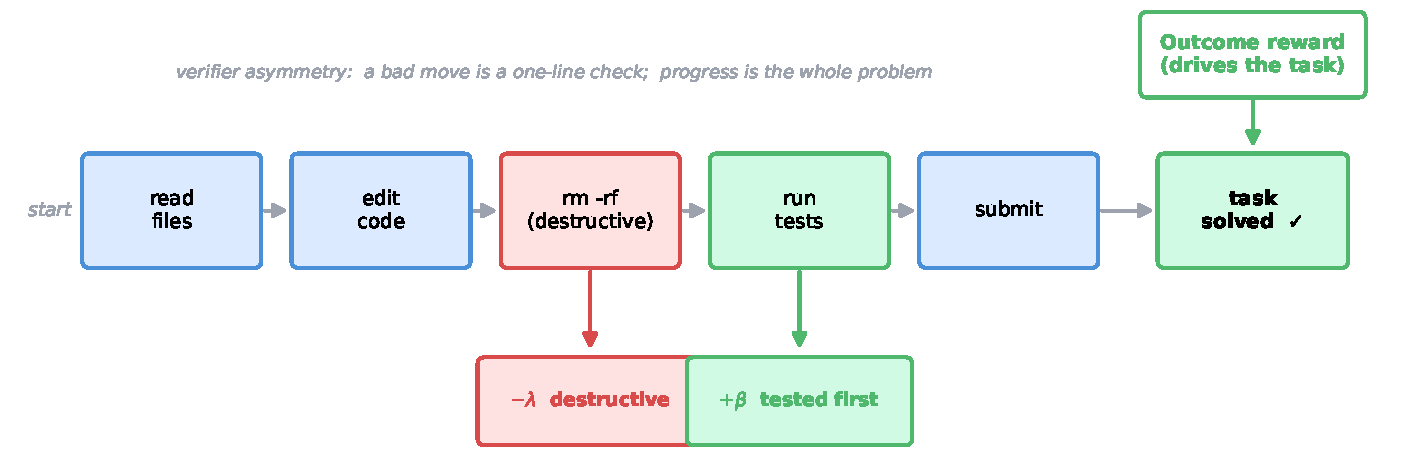
\includegraphics[width=\textwidth]{figures/fig_two_channel.pdf}
\caption{\textbf{Reward the outcome, penalize the path.} RLVR trains on the terminal outcome (right), which is blind to everything that happens along the trajectory. Agentic environments verify the \emph{path} asymmetrically: they cheaply flag bad actions (a destructive command, a call without its precondition) but cannot certify progress. RLVP adds a second, per-action channel that penalizes those verifiable bad moves and discharges the compliant ones. The outcome channel drives the task; the penalty channel teaches the outcome-neutral constraints the outcome cannot see.}
\label{fig:twochannel}
\end{figure}


\section{Background and When a Process Signal Helps}
\label{sec:background}

\paragraph{Group-relative RL.} Modern agentic RL largely dispenses with a learned value function and estimates advantages by comparison \emph{within a group} of rollouts of the same task~\citep{deepseekmath,deepseekr1}. For a prompt, one samples a group of $G$ trajectories, scores each with a reward, and sets each trajectory's advantage to its reward minus the group mean (often divided by the group standard deviation). There is no critic: the other members of the group \emph{are} the baseline. This is what makes verifiable rewards so effective---a rule or a test suite scores a trajectory directly---and it is the setting for everything that follows.

\paragraph{The advantage is a within-group variance.} Because the baseline is the group mean, a trajectory contributes gradient only to the extent its reward \emph{differs} from its group-mates. If every rollout in a group receives the same reward, all advantages are zero and the group produces no update. Under a binary outcome reward this happens in two regimes (Figure~\ref{fig:variance}): the \emph{all-fail} groups that dominate early training on long-horizon tasks, and the \emph{all-succeed} groups that dominate once a task is nearly solved. Group-relative RL is thus blind at both extremes of the success rate---a fact the field half-acknowledges by \emph{discarding} such groups (dynamic sampling in DAPO drops prompts that are all-correct or all-wrong~\citep{dapo}) rather than filling them with signal.

\paragraph{When a dense signal can help.} A dense process signal is useful exactly when it restores variance the outcome has lost. Writing the shaped reward as outcome plus $\beta$ times a process term, the group's reward variance decomposes into the outcome's variance, the process term's within-group variance, and their covariance. On an all-fail (or all-success) group the first term is zero, so \emph{all} usable gradient must come from the process term's own within-group variance. This gives a single, checkable condition: a process signal helps only where its within-group variance is nonzero---and that variance is realized only if the policy actually \emph{reaches} differing intermediate states across the group. Two very different signals meet or miss this condition in opposite ways. A verifiable \emph{penalty} on bad actions almost always carries variance: early in training some rollouts take the bad action and some do not, and both are cheap to sample and to check. A dense progress \emph{potential} carries variance only when the policy reaches partial success---which, on the hard tasks where all-fail groups dominate, it usually does not. The rest of the paper is this observation, made concrete: penalties are the reliable half of the process signal, potentials the fragile half.

\begin{figure}[t]
\centering
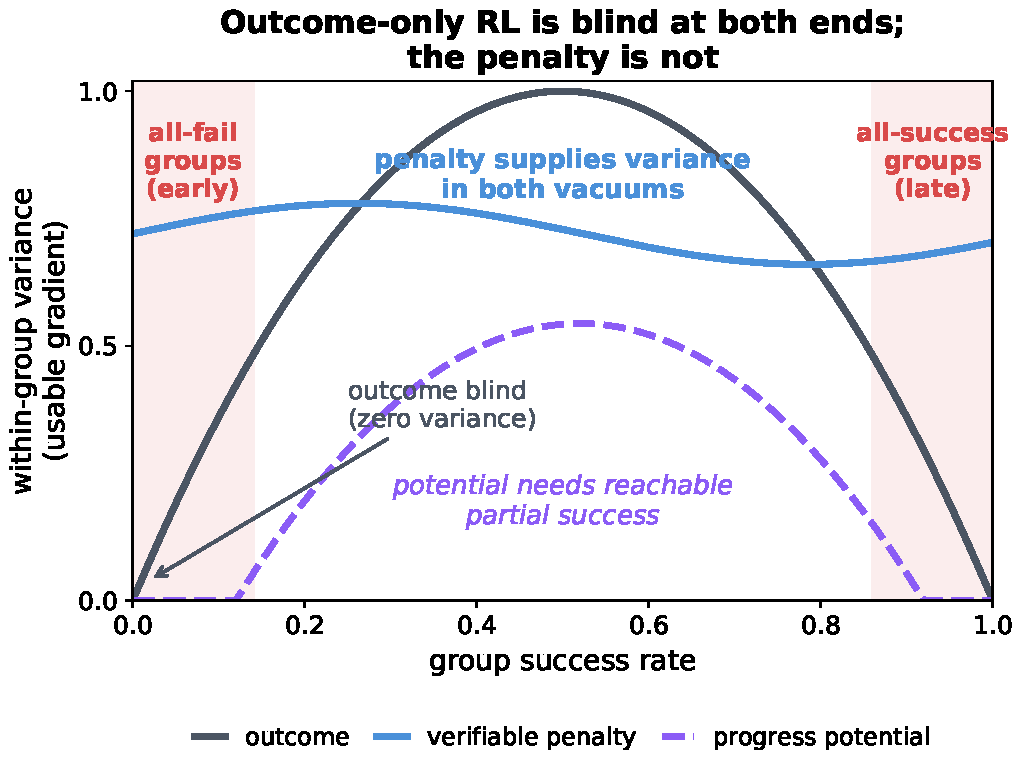
\includegraphics[width=\textwidth]{figures/fig_variance_vacuum.pdf}
\caption{\textbf{Outcome-only RL is blind at both ends of the success rate.} A group-relative advantage is a within-group variance, which the binary outcome drives to zero on all-fail groups (early training) and all-succeed groups (late training). A dense process signal helps only by supplying within-group variance in these vacuums---and only where the policy reaches the intermediate states that carry it. A verifiable penalty (bad moves are easy to sample) meets this reliably; a dense progress potential (partial success is rare on hard tasks) does not.}
\label{fig:variance}
\end{figure}


\section{Penalizing the Path: Robust Harm Reduction with Verifiable Penalties}
\label{sec:path}

\paragraph{Two channels.} We keep the outcome reward and add a second, per-action channel (Figure~\ref{fig:twochannel}). At each step, a deterministic rule engine---a pure predicate over the state before the step and the action taken---checks the action. A \emph{violation} (a destructive command, a call issued before its required precondition) attaches a penalty $-\lambda$ to that action's tokens; a \emph{discharge} of a pending obligation (performing the precondition) attaches a credit $+\beta$. The two channels are normalized separately, so the sparse path signal is not diluted or cancelled by the outcome channel, then combined. ``Penalize the path'' is therefore literal: the gradient lowers the probability of the specific offending action, in the specific context where it occurred, while the outcome channel scales whole trajectories by success. Crucially, the rules we penalize are \emph{outcome-neutral}---following or breaking them does not change whether the task is solved---so this is signal the outcome reward can never provide.

\paragraph{The recipe attains the task with near-zero violations.} On a suite of diverse system-administration and customer-service tasks with outcome-neutral rules, drawn from a large pool and evaluated on held-out instances, outcome-only training learns to \emph{solve} the tasks but violates the rules on essentially every episode: the constraints are invisible to its reward. Adding the penalty channel---reward the outcome, penalize the path---drives violations to near zero while keeping task success high, robustly across seeds and across model scales (Figure~\ref{fig:recipe}). The agent does not achieve this by going quiet: it takes as many actions as before, simply cleaner ones. This is the positive result in its cleanest form: a verifiable penalty teaches a real, deployable behavior---following the protocol---that the outcome reward cannot.

\begin{figure}[t]
\centering
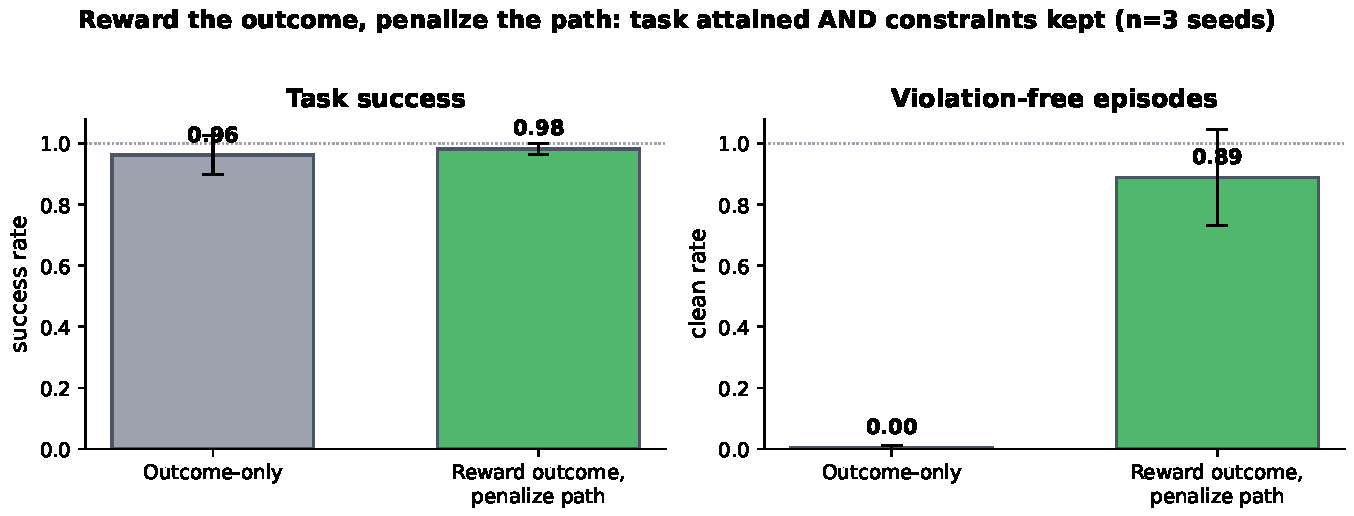
\includegraphics[width=\textwidth]{figures/fig_recipe_positive.pdf}
\caption{\textbf{Reward-the-outcome-penalize-the-path attains the task \emph{and} the constraints.} Across diverse held-out tasks and model scales, outcome-only training solves the task but violates the outcome-neutral rules on nearly every episode (low ``clean'' rate). The two-channel recipe keeps task success high while driving violation-free episodes to near-100\%, with small seed variance. Numbers are means over five seeds; error bars are one standard deviation.}
\label{fig:recipe}
\end{figure}

\paragraph{It transfers to a real agentic benchmark.} The synthetic domains let us control the rules; to test the same mechanism in the wild we train on TerminalBench, where each turn is a shell command in a task's container and the environment flags destructive actions. Task success there is at the floor for a small model, which makes it a clean test of the harm axis alone: at \emph{equal} task success, the harm penalty cuts destructive actions several-fold relative to outcome-only training, while the policy issues \emph{more} productive commands, not fewer (Table~\ref{tab:harm}, five seeds). The reduction is large relative to its variance---the per-seed distributions do not overlap---and it is not passivity. A verifiable penalty bounds the path independently of whether the task is solved, which is exactly the property a deployable agent needs.

\begin{table}[tbp]
\centering
\caption{\textbf{Harm reduction at equal outcome (TerminalBench, Qwen3-4B, 3 seeds, mean $\pm$ std).} Task success is identical and at the floor (4B rarely solves the benchmark), yet the un-gameable harm penalty cuts harmful actions roughly fourfold. The policy is not going passive: it takes about three times \emph{more} productive actions while violating less. Harm lives on an axis the terminal outcome cannot see.}
\label{tab:harm}
\small
\renewcommand{\arraystretch}{1.2}
\begin{tabular}{@{}lcc@{}}
\toprule
& \textbf{RLVP (harm penalty)} & \textbf{Outcome-only} \\
\midrule
Task success & $0.097 \pm 0.069$ & $0.097 \pm 0.063$ \;(equal, at floor) \\
\textbf{Violations / episode} & $\mathbf{0.95 \pm 0.71}$ & $3.99 \pm 0.57$ \\
Productive actions / episode & $\sim$\textbf{14} & $\sim$4 \\
\bottomrule
\end{tabular}
\end{table}



\section{Design Principles for Verifiable Penalties}
\label{sec:design}

A penalty is powerful but easy to misuse. The variance account and our ablations (Figure~\ref{fig:ablation}) yield four rules that, together, are the difference between the robust behavior above and a policy that stops working (Figure~\ref{fig:design}).

\paragraph{1. Penalize verifiable \emph{actions}, not lack of progress.} A good penalty targets a specific machine-checkable bad action---\emph{a} destructive command, \emph{a} call without its precondition. It must not target the \emph{absence} of progress (``penalize an unproductive step''), because the cheapest way to make no unproductive steps is to make no steps. Penalize commission, never omission.

\paragraph{2. Keep the outcome reward as the task driver; never optimize a penalty alone.} A penalty cannot be the primary learning signal. In the all-fail regime it is often the \emph{only} signal with any slope, and its cheapest maximizer is to stop acting: the policy drifts into a penalty-free, useless optimum---the \emph{inaction trap}. Our sweep makes this concrete: a pure penalty with no accompanying reward collapses to zero task success on every seed (Figure~\ref{fig:ablation}). The outcome reward is what forces the agent to keep acting; the penalty only shapes \emph{how}. Reward the outcome, and the penalty becomes a passenger that steers rather than an engine that stalls.

\paragraph{3. Pair the penalty with a discharge.} A penalty says only what \emph{not} to do. Adding a discharge---a $+\beta$ credit for performing the compliant action---gives a positive pull \emph{toward} doing it right, so the policy escapes the neighborhood of the bad action instead of merely avoiding it. Removing the discharge measurably slows and destabilizes the acquisition of compliant behavior (Figure~\ref{fig:ablation}).

\paragraph{4. Make the compliant behavior reachable and its target un-gameable.} A discharge can only reward behavior the policy actually samples; if the compliant path is never explored, no amount of shaping fires. Seeding training with a few scripted-compliant demonstrations supplies that reachability, after which the shaping can be annealed off once compliance saturates. And the penalized (and discharged) target must be the real action, not a learnable or hand-wavy proxy: a \emph{learned} judge of ``compliance'' simply relocates the hack into the judge, which the policy then games (Appendix~\ref{app:boundaries}).

Together these rules describe a narrow but reliable regime. The penalty is verifiable and outcome-neutral; it accompanies rather than replaces the outcome reward; it is paired with a discharge; and its target is reachable and un-gameable. The ablation in Figure~\ref{fig:ablation} walks a policy from outcome-only, through a pure penalty (the inaction trap) and penalty-plus-discharge, to the full recipe, and the compliant-and-successful behavior appears only when all four rules hold.

\begin{figure}[t]
\centering
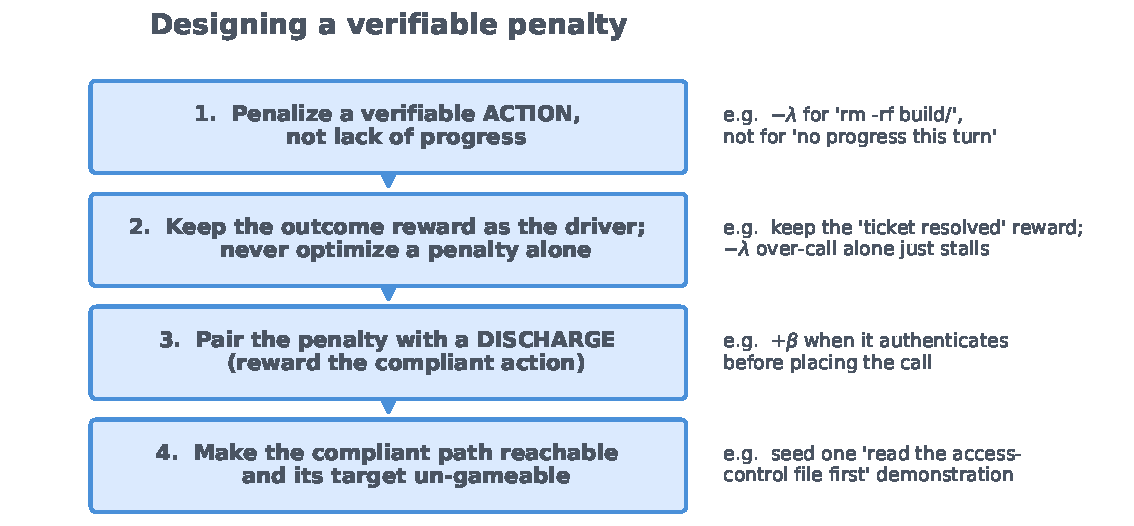
\includegraphics[width=0.9\textwidth]{figures/fig_penalty_design.pdf}
\caption{\textbf{A design procedure for verifiable penalties.} Before adding a penalty, a practitioner can check each rule in turn. Is there a verifiable \emph{action} to penalize (not an absence of progress)? Is the outcome reward still the task driver? Is the penalty paired with a discharge for the compliant action? Is that compliant action reachable, and its target un-gameable? Only when all four hold does the penalty bound the path without stalling the task.}
\label{fig:design}
\end{figure}

\begin{figure}[t]
\centering
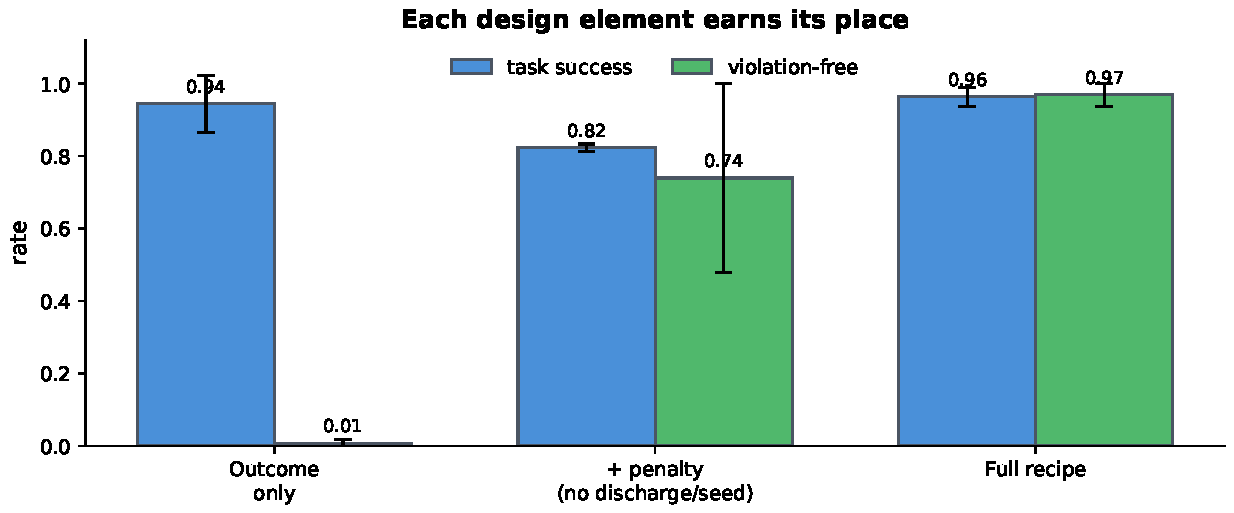
\includegraphics[width=\textwidth]{figures/fig_penalty_ablation.pdf}
\caption{\textbf{Each rule earns its place.} Removing a design element degrades the outcome. Outcome-only leaves violations high; a \emph{pure} penalty (no reward, no discharge) collapses to zero success---the inaction trap; penalty-plus-discharge without seeded reachability is seed-fragile; the full recipe attains high success \emph{and} near-zero violations. Five seeds; bars show mean, whiskers one standard deviation.}
\label{fig:ablation}
\end{figure}


\section{The Fragility of Dense Potentials}
\label{sec:potentials}

Why not shape with a dense progress \emph{potential} instead---rewarding the fraction of a proof completed, of tests passed, of stages cleared? The variance account predicts this is the fragile half of the process signal, and our experiments bear it out. The potential only supplies gradient where the policy reaches its intermediate values, and on the hard tasks where a dense signal is most wanted, it does not. On software repair the natural potential is the fraction of hidden tests an episode makes pass; across many rollouts of a capable model, \emph{every} episode makes zero tests pass, so the potential's within-group variance is identically zero and it centers out to nothing (Figure~\ref{fig:potentials}). This reachability, moreover, can be measured before training from a handful of base-policy rollouts, and the benefit of a dense potential tracks it.

Where the potential \emph{is} reachable, it does supply gradient---but the resulting efficiency gains are not robust. A dense potential that appears to reach a hard theorem-proving benchmark several times faster than outcome-only training reverses under re-seeding: with the sampler's randomness unfixed, the same configuration that ``wins'' on one run loses on the next, so even the \emph{sign} of the speed-up is not reproducible (Figure~\ref{fig:potentials}). This is the agentic-process-reward instance of a broader fragility now documented for RLVR~\citep{sober,spurious}, and a sharper one. We therefore do not build the paper on a potential's speed-up. The reliable use of the verifier is the penalty; the potential's promise of acceleration is, at present, a lottery. Full experiments are in Appendix~\ref{app:potentials}.

\begin{figure}[t]
\centering
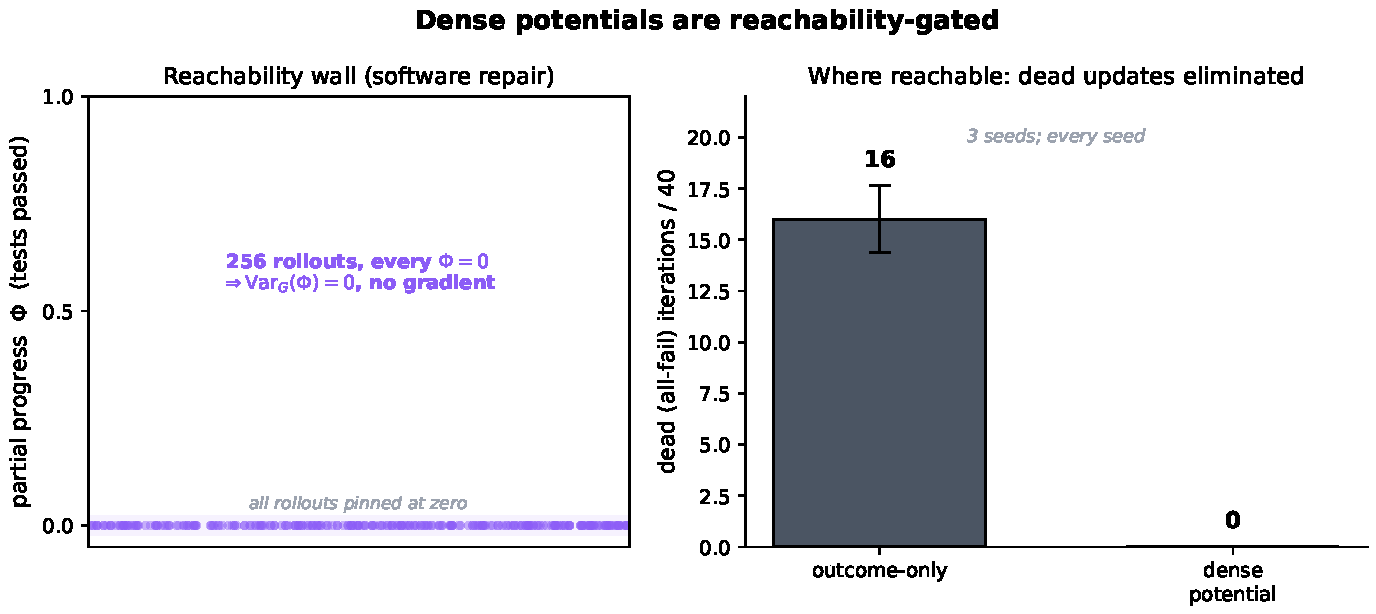
\includegraphics[width=\textwidth]{figures/fig_potential_fragility.pdf}
\caption{\textbf{Dense potentials are reachability-gated and fragile.} \emph{Left:} on software repair the finer potential is unreachable---across many rollouts the policy makes zero partial progress, so its within-group variance is zero and it gives no gradient. \emph{Right:} where a potential is reachable its apparent speed-up does not survive re-seeding---the same configuration reverses sign across runs. The reliable half of the process signal is the penalty, not the potential.}
\label{fig:potentials}
\end{figure}


\section{Discussion}

\paragraph{Verifier asymmetry as a design principle.} The practical takeaway is a reallocation. A verifier is a scarce, valuable thing, and the field has been spending it on the direction it is worst at---certifying progress---while avoiding the direction it is best at---catching bad moves. Spend it on penalties. When there is an outcome-neutral constraint a deployed agent must respect, and a verifiable bad action to attach it to, a penalty paired with a discharge and wired alongside the outcome reward will teach it, robustly and cheaply. When the only dense signal available is a progress proxy, expect a lottery, and prefer to simply reward the outcome.

\paragraph{A systems note.} The property that makes a verifiable penalty cheap---a machine-checkable environment---tends to make the verifier a CPU process (a rule engine, a test runner, a container). In our theorem-proving runs the accelerator generated a step in milliseconds and then waited seconds on the proof kernel, leaving GPU utilization in the single digits at full memory (Figure~\ref{fig:verifier}). This is workload-dependent, not a law, but for the verifiable domains where penalties apply, throughput is gated by environment parallelism, and the right systems design co-locates many verifier workers per accelerator rather than scaling accelerators.

\paragraph{Limitations.} Our cleanest real-task harm result is measured where task success is at the floor; the mechanism predicts it holds at higher success (a penalty's variance is reachable regardless of success), but demonstrating that on a capable model is the natural next step. Our penalties are hand-identified per domain from the environment's rules; automating their discovery from an environment's affordances is open. And the un-gameability sweep that anchors the inaction-trap result is high-variance at scale; we report its \emph{survival pattern} rather than precise magnitudes.

\begin{figure}[t]
\centering
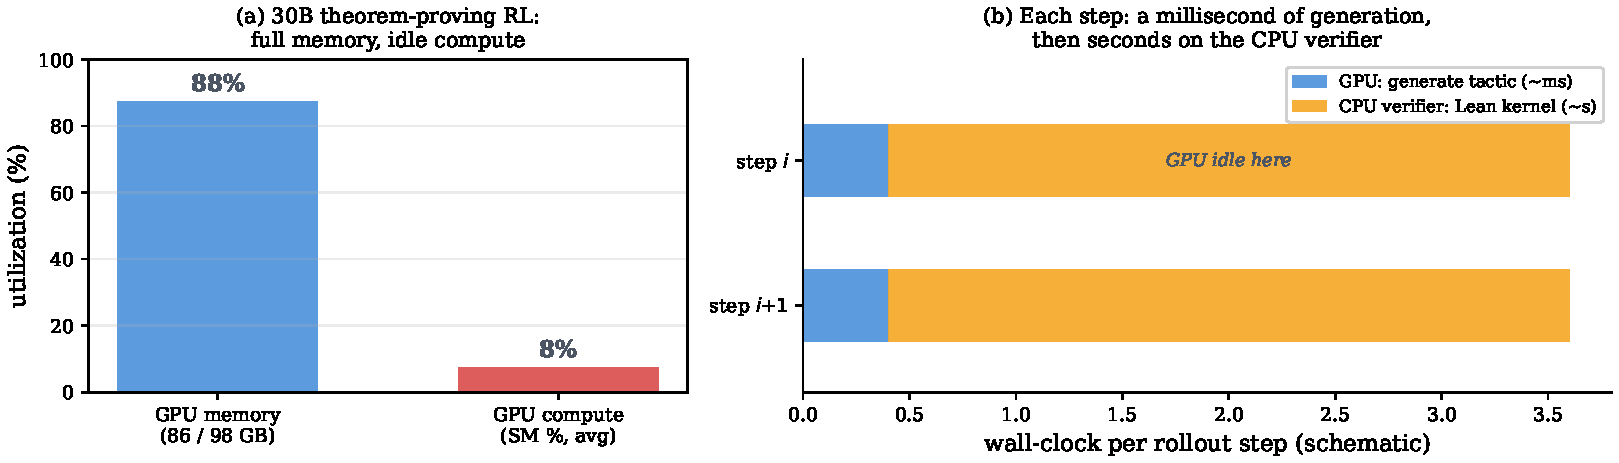
\includegraphics[width=0.9\textwidth]{figures/fig_verifier_bound.pdf}
\caption{\textbf{Verifiable agentic RL is often verifier-bound.} In theorem-proving runs the GPU sits near-idle at full memory while the CPU proof kernel checks each step. The signal that makes a penalty cheap also moves the bottleneck off the accelerator.}
\label{fig:verifier}
\end{figure}


\section{Related Work}

\paragraph{Group-relative RL and the zero-variance problem.} Agentic RL has largely converged on GRPO~\citep{deepseekmath} and the rule-based R1 line~\citep{deepseekr1,tulu3}, which replace the value critic with a within-group baseline. Under binary verifiable rewards, an output's advantage is then \emph{definitionally} a within-group variance, and it collapses to zero whenever a group is uniformly solved or uniformly failed. The field has named this ``advantage collapse'' and responded in four ways: DAPO~\citep{dapo} \emph{discards} zero-variance prompts via dynamic sampling, keeping only groups with $0<\#\text{correct}<G$; Dr.\,GRPO~\citep{drgrpo} \emph{removes} the difficulty-dependent standard-deviation normalizer; GSPO~\citep{gspo} \emph{stabilizes} the importance ratio at sequence level; and RL-ZVP~\citep{rlzvp} \emph{manufactures} a signal in zero-variance groups from output entropy. Notably, DAPO discards \emph{all-correct} groups as well as all-wrong ones---an implicit acknowledgment that group-relative RL is blind at \emph{both} extremes. We make the symmetry explicit and, rather than dropping the blind groups, ask which dense signal can \emph{supply} the missing variance---finding that a verifiable penalty reliably can and a dense potential reliably cannot.

\paragraph{Process reward models and their gameability.} Step-level supervision outperforms outcome supervision for verification~\citep{prm}, with per-step labels obtainable automatically via Monte-Carlo rollouts~\citep{mathshepherd}. \citet{setlurprogress} argue the useful process signal is a progress measure---a step-level advantage---closely paralleling our variance view, but instantiate it with a \emph{learned} prover. A consistent body of evidence shows learned dense rewards are hacked under RL pressure: over-optimization follows clean Goodhart laws~\citep{overopt}, capable agents exploit misspecification harder~\citep{misspec}, summation-form PRM credit induces RL collapse~\citep{pure}, and learned value credit is unreliable~\citep{vineppo}. DeepSeek-R1~\citep{deepseekr1} abandoned PRMs because a model-based PRM ``inevitably leads to reward hacking,'' while \citet{freeprm} show an outcome reward model implicitly contains a PRM. We take these as motivation for a \emph{verifiable, non-learned} penalty that cannot be gamed by construction, and as evidence for our fourth design rule.

\paragraph{Potential-based shaping: safe versus useful.} \citet{ng1999} prove potential-based shaping leaves the optimal policy unchanged for \emph{any} potential, and \citet{wiewiora2003} show such shaping equals value initialization---it affects learning dynamics, not the fixed point. This certifies which dense signals are \emph{safe}, not which are \emph{useful}. Our account is orthogonal to the safety guarantee: among safe shapings, the useful ones supply within-group variance the outcome lacks, and only where reachable---which is why a penalty on always-sampled bad actions helps and a potential on rarely-reached progress does not.

\paragraph{Process rewards in agentic RL, and the fragility of RL gains.} Step- and turn-level credit for agents has been explored via hierarchical critics~\citep{archer}, learned step rewards~\citep{steptool,sparl}, and turn-level advantage estimators~\citep{turnlevel}; the closest to a verifiable signal are GiGPO~\citep{gigpo} and per-tool-call correctness~\citep{toolrl}. Verifiable \emph{outcome} rewards underpin agentic benchmarks and training~\citep{taubench,tau2bench,swegym,swerl}. \citet{practitioner} find dense turn-level rewards \emph{accelerate} training but their effect on final performance depends on the policy-gradient estimator. This aligns with a broader reproducibility literature: pass@1 varies by up to $\sim$15\% across seeds~\citep{sober}, random rewards can ``improve'' some models through optimization bias~\citep{spurious}, one example suffices for much of the gain~\citep{oneshot}, and at large $k$ base models match RLVR models~\citep{rlbeyond}. Our potential result is the agentic-process-reward instance of this fragility, and sharper: even the \emph{sign} of the speed-up flips under re-seeding. Learned-judge rewards~\citep{selfreward,rlaif,constitutional,llmjudge} and off-policy demonstration mixing~\citep{luffy} are complementary; our fourth design rule uses the latter for reachability and warns against the former for un-gameability.


\section{Conclusion}

RLVR taught language agents from the one bit an environment checks cheaply---the final outcome. The instinct to go denser has been to reward the process, but the environment cannot verify progress; it can only verify mistakes. The dense signal it actually affords is a penalty on the path, not a reward on progress. Wired correctly---alongside the outcome reward, paired with a discharge, aimed at a reachable and un-gameable target---a verifiable penalty teaches the outcome-neutral constraints that make an agent deployable, robustly and across scales, while a lone penalty stalls and a dense potential is a lottery. The contribution is not a new optimizer but a reallocation of a scarce resource: spend the verifier on penalties that bound the path, and let the outcome reward do what it already does---teach the task.
